% Created 2024-04-16 Tue 14:54
% Intended LaTeX compiler: pdflatex
\documentclass[presentation]{beamer}
\usepackage[utf8]{inputenc}
\usepackage[T1]{fontenc}
\usepackage{graphicx}
\usepackage{longtable}
\usepackage{wrapfig}
\usepackage{rotating}
\usepackage[normalem]{ulem}
\usepackage{amsmath}
\usepackage{amssymb}
\usepackage{capt-of}
\usepackage{hyperref}
\mode<beamer>{\usetheme{Madrid}}
\definecolor{SUred}{rgb}{0.59375, 0, 0.17969} % SU red (primary)
\definecolor{SUblue}{rgb}{0, 0.17578, 0.38281} % SU blue (secondary)
\setbeamercolor{palette primary}{bg=SUred,fg=white}
\setbeamercolor{palette secondary}{bg=SUblue,fg=white}
\setbeamercolor{palette tertiary}{bg=SUblue,fg=white}
\setbeamercolor{palette quaternary}{bg=SUblue,fg=white}
\setbeamercolor{structure}{fg=SUblue} % itemize, enumerate, etc
\setbeamercolor{section in toc}{fg=SUblue} % TOC sections
% Override palette coloring with secondary
\setbeamercolor{subsection in head/foot}{bg=SUblue,fg=white}
\setbeamercolor{date in head/foot}{bg=SUblue,fg=white}
\institute[SU]{Shenandoah University}
\titlegraphic{\includegraphics[width=0.5\textwidth]{\string~/Documents/suLogo/suLogo.pdf}}
\newcommand{\R}{\mathbb{R}}
\usepackage{tikz}
\usepackage{pgfplots}
\usetheme{default}
\author{Chase Mathison\thanks{cmathiso@su.edu}}
\date{17 April 2024}
\title{The Ellipse}
\hypersetup{
 pdfauthor={Chase Mathison},
 pdftitle={The Ellipse},
 pdfkeywords={},
 pdfsubject={},
 pdfcreator={Emacs 29.1 (Org mode 9.6.7)}, 
 pdflang={English}}
\begin{document}

\maketitle

\section{Announcements}
\label{sec:org0bfbd6a}
\begin{frame}[label={sec:orgf0c39b5}]{Announcements}
\begin{enumerate}
\item Office hours today 10am - 11am.
\item Homework in MyOpenMath, and Projects (2 of them).
\end{enumerate}
\end{frame}

\section{Lecture}
\label{sec:org7a36c37}
\begin{frame}[label={sec:org40c14dc}]{The ellipse}
An ellipse is defined in the following strange way:

\begin{definition}[Ellipse]
Given two points \(F_1\) and \(F_2\) (called \uline{\hspace*{1in}}) that are not the same point in
the \(xy-\)plane, an ellipse is the set of all \(\left( x,y \right)\)
such that the sum of the distances from \(\left( x,y \right)\) to
\(F_1\) and \(\left( x,y \right)\) to \(F_2\) is a \uline{\hspace*{1in}} value.
\end{definition}
\end{frame}

\begin{frame}[label={sec:orga52d7a7}]{The ellipse}
There's a lot to unpack here, so let's get to unpacking!

\begin{tikzpicture}
  \begin{axis}[axis lines = center,
    xmin = -4,
    xmax = 4,
    ymin = -4,
    ymax = 4,
    xlabel = {$x$},
    ylabel = {$y$}]
    
  \end{axis}
\end{tikzpicture}
\end{frame}

\begin{frame}[label={sec:orgdf2beaf}]{Some key features}
\begin{description}
\item[{Major axis}] 

\item[{Minor axis}] 

\item[{Vertex}] 

\item[{Co-vertex}] 

\item[{Center of ellipse}] 
\end{description}

\vspace{1in}  
The foci always lie on the \uline{\hspace*{1in}} axis.
\end{frame}

\begin{frame}[label={sec:org6183e1a}]{Deriving the formula for an Ellipse}
\begin{tikzpicture}[scale=1]
  \begin{axis}[axis lines = center,
    xmin = -4,
    xmax = 4,
    ymin = -4,
    ymax = 4,
    xlabel = {$x$},
    ylabel = {$y$}]
    
  \end{axis}
\end{tikzpicture}
\end{frame}

\begin{frame}[label={sec:org65e0e94}]{Deriving the formula for an Ellipse}
\end{frame}

\begin{frame}[label={sec:org967d665}]{Facts about Ellipses centered at the Origin}
\begin{center}
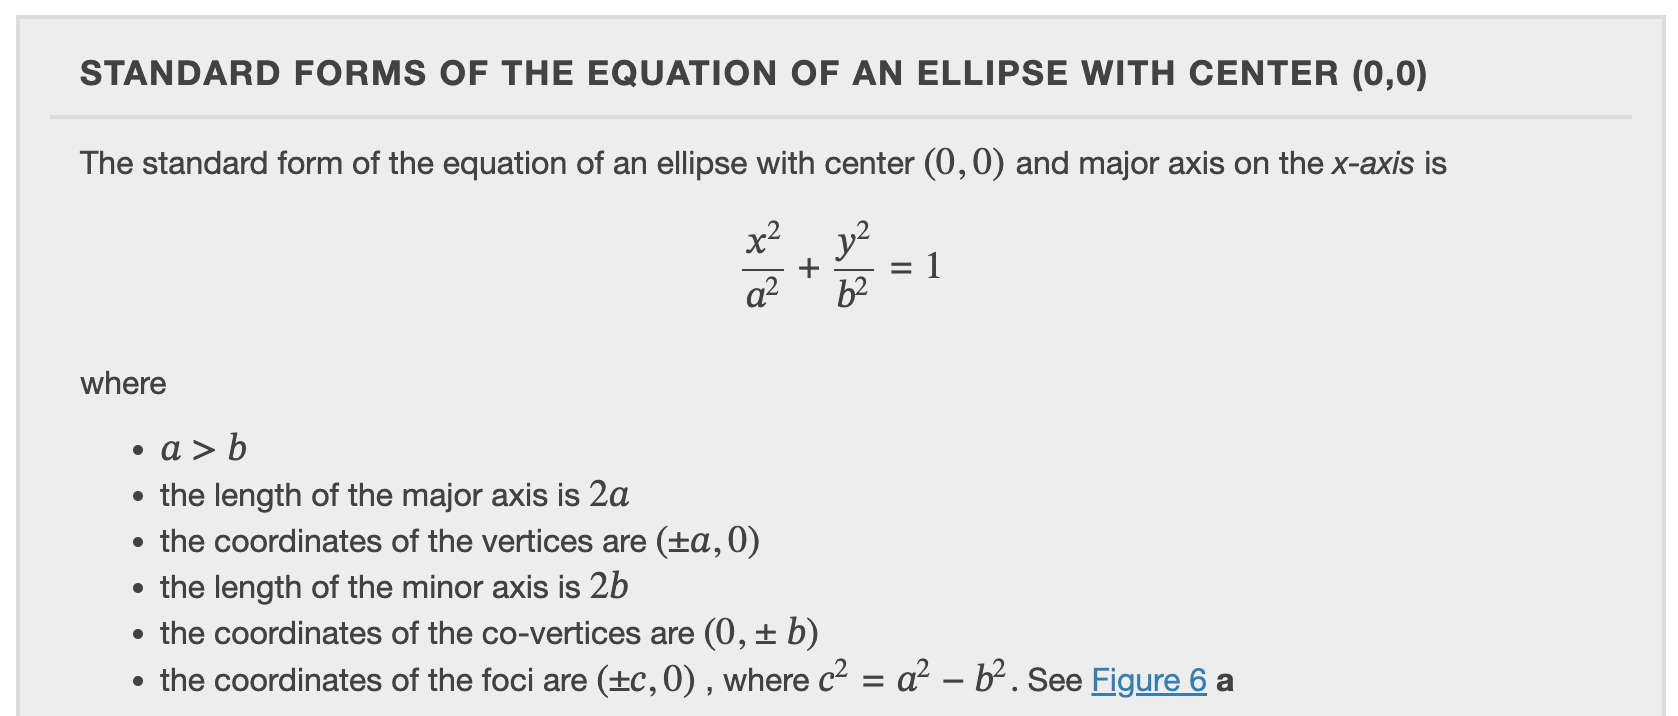
\includegraphics[width=0.8\textwidth]{./ell01.png}
\end{center}
\end{frame}

\begin{frame}[label={sec:orgb8619f9}]{Facts about Ellipses centered at the Origin}
\begin{center}
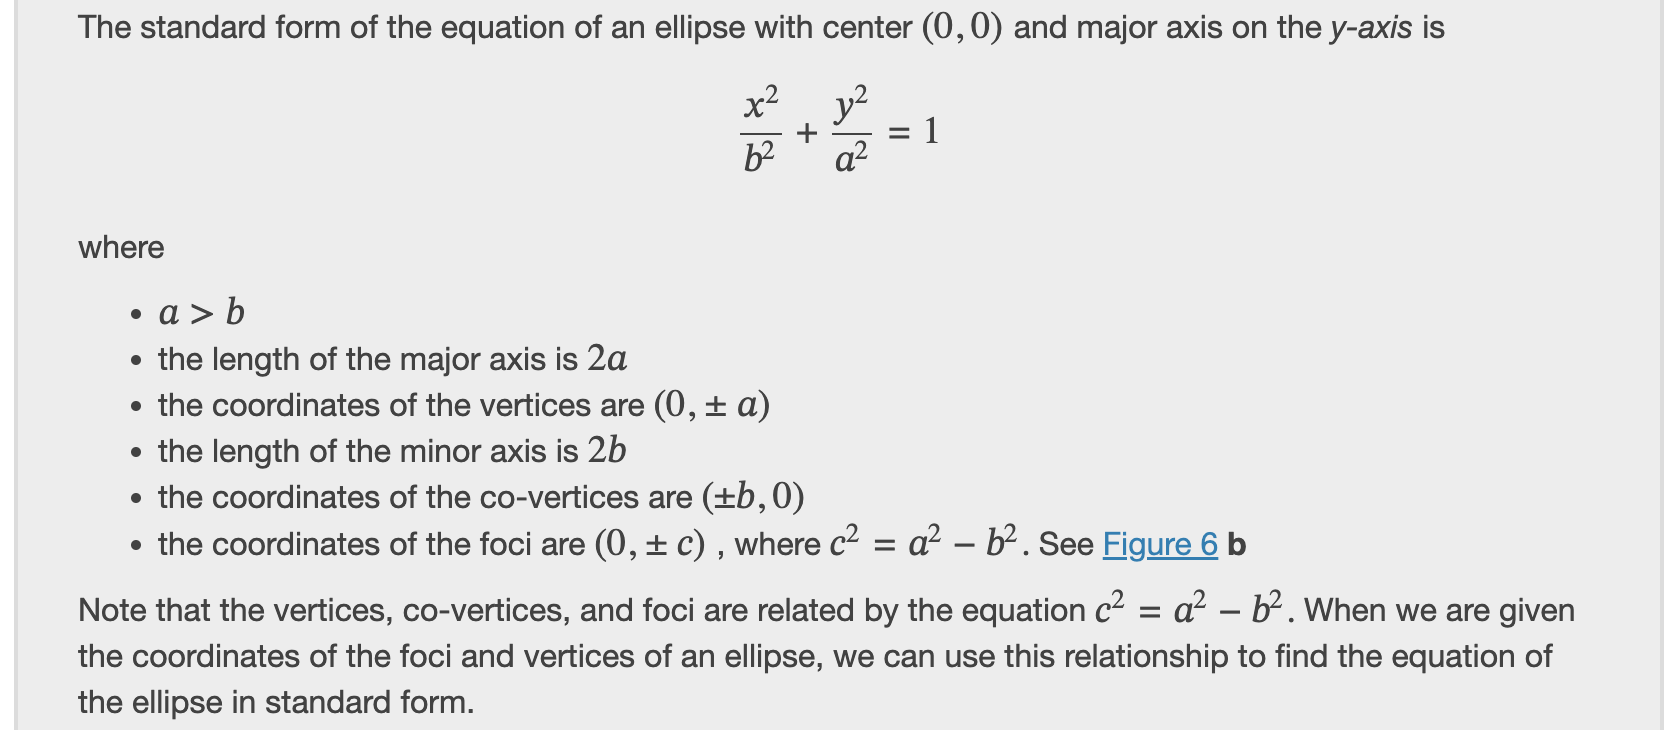
\includegraphics[width=0.8\textwidth]{./ell02.png}
\end{center}
\end{frame}

\begin{frame}[label={sec:org5a8991b}]{Facts about Ellipses centered at the Origin}
\begin{center}
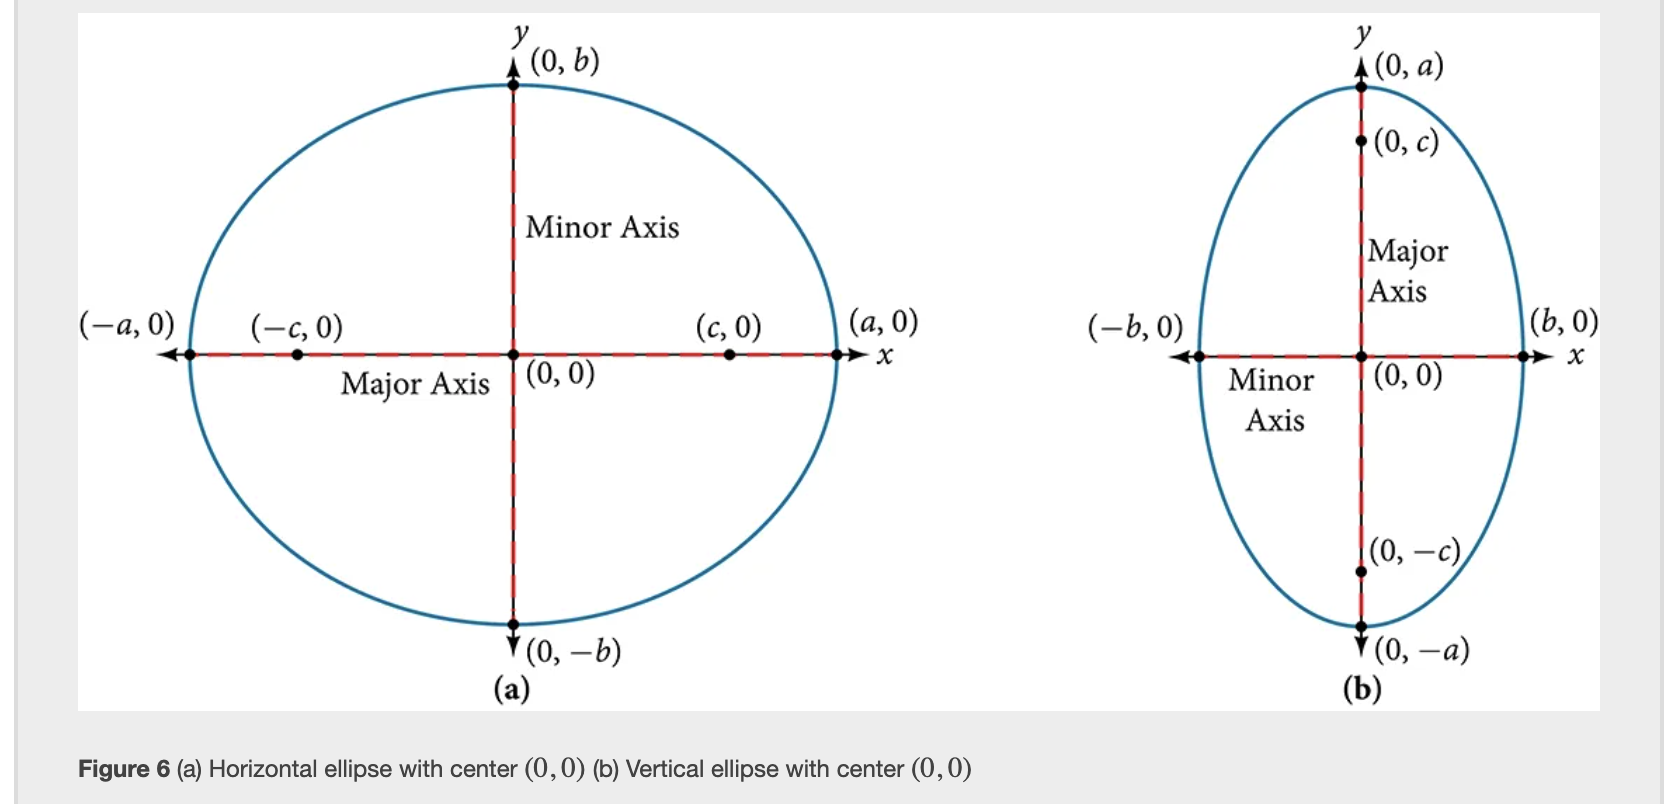
\includegraphics[width=0.8\textwidth]{./ell03.png}
\end{center}
\end{frame}

\begin{frame}[label={sec:org271777c}]{Example}
Write the equation of the following ellipse and identify the key features of the ellipse.

\begin{tikzpicture}[scale=1]
  \begin{axis}[axis lines = center,
    xmin = -4,
    xmax = 4,
    ymin = -4,
    ymax = 4,
    xlabel = {$x$},
    ylabel = {$y$}]

    \addplot[domain=-3:3,samples=500]{sqrt(1-x^2/9)};
    \addplot[domain=-3:3,samples=500]{-sqrt(1-x^2/9)};
  \end{axis}
\end{tikzpicture}
\end{frame}

\begin{frame}[label={sec:orge54e7f7}]{Example}
\end{frame}

\begin{frame}[label={sec:org1598737}]{Example}
Write the equation of the following ellipse and identify the key features of the ellipse.

\begin{tikzpicture}[scale=1]
  \begin{axis}[axis lines = center,
    xmin = -4,
    xmax = 4,
    ymin = -4,
    ymax = 4,
    xlabel = {$x$},
    ylabel = {$y$}]

    \addplot[domain=-2:2,samples=500]{4*sqrt(1-x^2/4)};
    \addplot[domain=-2:2,samples=500]{-4*sqrt(1-x^2/4)};
  \end{axis}
\end{tikzpicture}
\end{frame}

\begin{frame}[label={sec:org8796b62}]{Example}
\end{frame}
\end{document}